% N.B. : Assurez-vous de compiler ce fichier en employant "pdflatex" afin que les images soient incluses.

% Tout commentaire est bienvenu et devrait être adressé à "support@dms.umontreal.ca".

    % L'appel de \Requireackage{natbib} est fait dans dms.cls si \documentclass est appelé
    % avec l'option <natbib>.  Les options de <natbib> sont données ici.
    % Vous pouvez les modifier, p.ex. ajouter <round> si vous préférez des parenthèse (1) 
    % plutôt que des crochets [1].
\PassOptionsToPackage{longnamesfirst,numbers}{natbib}  
\documentclass[12pt,maitrise,frenchb,natbib,twoside,initial]{dms} 
% La commande précédente charge la classe "dms.cls" avec les options suivantes : 
%   -police de caractères en 12 pts 
%   -format adapté à une thèse de doctorat 
%   -écriture française (par défaut avec la classe)
%   -impression recto-verso.
%   -adapté pour le dépôt initial (enlever l'option pour le dépôt final)
%
% Modifiez cette commande selon vos besoin à l'aide des options suivants :
% maitrise			mémoire de maîtrise;
% phd				thèse de doctorat;
% phdart                        thèse de doctorat par articles;
% rapport			rapport de stage;
% travaildirige			travail dirigé;
% oneside			impression recto;
% twoside			impression recto-verso.
% initial			depot initial (sans l'option pour depot final)
% policeTNR                     pour utiliser (l'équivalent de) Times New Roman (sinon <lmodern> est chargé, la fonte par défaut)
% nobabel			document en anglais seulement
% frenchb			document en français
% frenchb,english		document contenant du français et de l'anglais (utiliser \selectlanguage{} )

%\usepackage[utf8]{inputenc}	% Fait dans le classe		
%\usepackage[T1]{fontenc}		

% La commande \sloppy peut avoir des effets étranges sur les
% lignes de certains paragraphes.  Dans ce cas, essayez \fussy
% qui suppresse les effets de \sloppy. (\fussy est le comportement par défaut.)
% On redéfinit \sloppy, pour tenter de réduire les comportements étranges.  
% Le seul changement apporté à la version originale est la valeur de \tolerance.
\def\sloppy{%
  \tolerance 500%  %9999 dans LaTeX ordinaire, mauvaise idée.
  \emergencystretch 3em%
  \hfuzz .5\csname p@\endcsname
  \vfuzz\hfuzz}
\sloppy  



\usepackage{graphicx,amsmath,amsfonts,amssymb,setspace,subfigure,color,icomma,dsfont}
% graphicx		Pour importer des images (PDF, JPG, PNG).
% amsmath		Écriture selon les normes de l'AMS.
% amsfonts		Fontes additionnelles de l'AMS.
% amssymb		Écriture des symbols de l'AMS.
% setspace		Permet de régler la distance interligne dans le document.
% subfigure		Simplifie l'inclusion de figures côtes-\`a-côtes.
% color			Pour l'utilisation de couleurs dans le texte.
% icomma		Reconnait la virgule comme caractère mathematique de facon intelligent
% dsfont		symboles mathématiques


\usepackage[pdfpagemode=UseNone,pdfstartview={XYZ null null null}]{hyperref}	% Cette extension permet l'insertion d'hyperliens dans votre document pdf.
 \definecolor{dark-red}{rgb}{0.4,0.15,0.15}					% Ici, trois couleurs sont définies et seront utilisées pour colorer les "hyperliens".
 \definecolor{dark-blue}{rgb}{0.15,0.15,0.4}
 \definecolor{medium-blue}{rgb}{0,0,0.5}
 \hypersetup{colorlinks,linkcolor={dark-red},citecolor={dark-blue},urlcolor={medium-blue}}
\usepackage{bookmark}  % Remédie à des petits problème de <hyperref> (important qu'il soit chargé après <hyperref>)
  % Enlever les commentaires et remplir cette section avec l'information pertinente.
  % Ceci ajoute des « méta-données » au pdf.  C'est optionnel, mais recommandé.
  % Vous pouvez voir ces méta-données en ouvrant un visionneur de pdf et en cherchant les
  % propriétés du pdf.  (Vous pouvez aussi tapez ' pdfinfo <nom-du-pdf> '  dans un terminal.)
  % Ces données sont utiles, par exemple, pour augmenter les chances qu'un algorithme de
  % recherche trouve votre document sur Internet, une fois diffusé.  Autrement dit, ceci
  % peut aider à augmenter la visibilité de votre travail.
%\hypersetup{
%    pdftitle = {Exemple d'une thèse}, 
%    pdfauthor = {Coadmin},
%    pdfsubject = {Exemple pour utiliser le gabarit du DMS},
%    pdfkeywords = {DMS, gabarit, exemple, thèse, mémoire, coadministrateur}
%}

% Numérotation des équations par section et numérotation des tableaux et figures par chapitre.
\numberwithin{equation}{section}
\numberwithin{table}{chapter}
\numberwithin{figure}{chapter}

% Définition des environnements utiles pour un mémoire scientifique.
% 1	%FR
\newtheorem{cor}{Corollaire}[section]
\newtheorem{deff}{Définition}[section]
\newtheorem{exemple}{Exemple}[section]
\newtheorem{lemme}{Lemme}[section]
\newtheorem{prop}{Proposition}[section]
\newtheorem{rem}{Remarque}[section]
\newtheorem{theo}{Théor\`eme}[section]

% Si vous préférez que les corollaires, definitions, théor\`emes, etc. soient numérotés par le même compteur, utilisez plutôt ce bloc de commandes : 
%2	% FR
%\newtheorem{corollary}{Corollaire}[section]
%\newtheorem{definition}[corollary]{Définition}
%\newtheorem{example}[corollary]{Exemple}
%\newtheorem{lemma}[corollary]{Lemme}
%\newtheorem{proposition}[corollary]{Proposition}
%\newtheorem{remark}[corollary]{Remarque}
%\newtheorem{theorem}[corollary]{Théor\`eme}


\onehalfspacing				% Fixe la distance interligne \`a "1.5". Pour une interligne double, utilisez plutôt "\doublespacing".

\allowdisplaybreaks			% Cette commande autorise LaTeX \`a briser les blocs d'équations, permettant ainsi une couverture plus uniforme des pages.

%Commande pour numéroter les tableaux en chiffres romains (préfixe: le numéro du chapitre)
\renewcommand{\thetable}{\thechapter. \Roman{table}}

%%%%%%%%%%%%%%%%%%%%%%%%%%%%%%%%%%%%%%%%%%%%%%%%%%%%%%%
% ---------  D É B U T  D U  D O C U M E N T  ---------
%%%%%%%%%%%%%%%%%%%%%%%%%%%%%%%%%%%%%%%%%%%%%%%%%%%%%%%
\begin{document}

% La commande "\brouillon" imprime, au bas de chaque page, la date ainsi que l'heure de la derni\`ere compilation de votre fichier.
%\brouillon            

% Voici les variables pour la création de votre page titre.

\title{Extraction des patrons de régime de VerbNet pour une implémentation dans un système de génération automatique de texte}
\author{Daniel Galarreta-Piquette}
\copyrightyear{2018}
\date{\today}									% Date de dépôt du document.
	% ces éléments ne doivent plus apparaittre selon les dierectives de la FESP
	% si toutefois vou souhaitez les inclure, il faudra aussi modifier le document dms.cls
% \president{Nom du président du jury}
% \directeur{Nom du directeur de recherche}
% \codirecteur{Nom du codirecteur}
% \membrejury{Nom du membre du jury} 
% \examinateur{Nom de l'examinateur externe}
% %\membresjury{ala, beta, gamma}
% %\plusmembresjury{psi, zeta, omega} 
% \repdoyen{Nom du représentant du doyen} 
\dateacceptation{Date d'acceptation}
\sujet{linguistique}							% Votre discipline de recherche, soit "mathématiques" ou "statistique".
%\orientation{mathématiques fondamentales}		% Cette commande est optionnelle. Les choix courants sont : "mathématiques fondamentales", "mathématiques de l'ingénieur" et "mathématiques appliquées".

\department{Département de traduction et linguistique}

% Fin des variables \`a définir. La commande "\maketitle" créera votre page titre.


\pagenumbering{roman}
\maketitle    
 
\chapter*{Sommaire} 	% La commande "\chapter*" crée un chapitre sans numéro, contrairement \`a la commande "\chapter" réguli\`ere.

% N.B. : La commande "\noindent" force LaTeX \`a ne pas indenter le nouveau paragraphe.
\noindent Ce mémoire explore les patrons de régime en anglais provenant de la ressource lexicographique \emph{VerbNet} et leur implémentation dans un système de génération automatique de texte. 	

\chapter*{Summary}

\noindent English summary and keywords\dots


% TABLE DES MATIÈRES
\cleardoublepage
\pdfbookmark[chapter]{\contentsname}{toc}  %Crée un bouton sur la bar de navigation
\tableofcontents				% Table des mati\`eres.
% LISTE DES TABLEAUX
\cleardoublepage
\phantomsection
\listoftables
% LISTE DES FIGURES
\cleardoublepage
\phantomsection
\listoffigures	


%%%%%%%%%%%%%%%%%%%%%%%%%%%%%%%%%%%%%
%% LISTE DES SIGLES ET ABRÉVIATION %
%%%%%%%%%%%%%%%%%%%%%%%%%%%%%%%%%%%%%
%% Il est obligatoire, selon les directives de la FESP, 
%% pour une thèse ou un mémoire d'avoir une liste des sigles et 
%% des abréviations.  Si vous considérez que de telles listes ne seraient pas
%% pertinentes (si, par exemple, vous n'utilisez aucun sigle ou abré.), son
%% inclusion ou omission est laissé à votre discrétion.  En cas de doute,
%% parlez-en à votre directeur de recherche, le coadministrateur ou, ultimement, à
%% la FESP directement.
%%
%% Dans le cas où vous incluez une table des sigles et des abréviations,
%% vous pouvez enlever les % de la section suivante pour faire apparaître
%% un exemple d'une telle liste « fait à la main ».  Il existe des outils
%% plus sophistiqués si vous devez inclure une multitude de sigles et abréviations.
%% (Par exemple, le package <glossaries> peut faire des index élaborés.  Comme
%% son utilisation est technique, il n'y a pas d'exemple directement dans ce gabarit.
%% On invite les gens qui aurait à l'utiliser à consulter le wiki
%% du dms, le coadministrateur ou faire leur propre recherche.)

\chapter*{Liste des sigles et des abréviations}
\begingroup %Pour que le \renewcommand soit local
%Modifiez ce nombre (p.ex.remplacez 2 par 1.5) pour augmenter ou diminuer l'espace entre les lignes du tableau.
\renewcommand{\arraystretch}{2} 
\noindent\begin{tabular}{p{.2\textwidth} p{.7\textwidth}}
  GAT & Génération automatique de texte \\
  GP & Patron de régime, de l'anglais \textit{Government Pattern}\\
  DPOS  &  Partie du discours profonde, de l'anglais \textit{Deep Part of Speech}\\
  TST & Théorie Sens-Texte\\
  VN & \emph{ VerbNet}\\
\end{tabular}
\endgroup  %Fin du groupe local pour \arraystretch


\chapter*{Dédicaces}

\vspace{2cm}
\hspace{2.5cm}Vos d\'edicaces.

\chapter*{Remerciements}

\noindent Remerciements\dots


% Fin des pages liminaires. À partir d'ici, les premi\`eres pages des chapitres ne doivent pas être numérotées.

% Voici maintenant le chapitre d'introduction.
\NoChapterPageNumber 


\chapter*{Introduction}

\pagenumbering{arabic}

\noindent Parler de la génération de texte automatique, de\emph{ VerbNet}, de la problématique (pas de consensus quant à l'architecture de la classe verbale dans des générateurs de texte automatiques) de verbnet, des lexicons 

% Ici débute le corps de votre texte.

\chapter{Extraction des entrées du lexicon \emph{Verbnet}}

%Le 1$^{\text{er}}$ chapitre numéroté. Voici quelques mots en \emph{italique}, en \textbf{gras} et \textsf{sans serif}.
Dans ce chapitre, nous verrons l'apport que la ressource lexicale \emph{VerbNet} peut offrir à des applications de TAL. L'objectif était d'extraire les patrons de régime qu'on retrouve dans le lexicon verbal VerbNet pour les implémenter au lexicon  de notre système de génération de texte automatique (GAT). Cet objectif provient d'une problématique que nous avions rencontré en travaillant sur l'architecture de la classe verbale dans notre système de GAT.  En ce qui concerne les lexicons, il ne semble pas y avoir de consensus quant à la manière de procéder pour former le lexicon quand vient le moment d'intégrer les entrées appartenant à la classe des verbes.  Les entrées lexicales faisant partie de cette partie du discours démontre des comportements variables, très riches, et assez complexes ce qui nécessite beaucoup plus d'attention que d'autres parties du discours comme les noms qui démontrent beauoup moins de variétés d'usage quant au nombre de patrons de régime. Cette problématique nous a donc amené à voir comment une ressource comme VerbNet qui s'est donnée comme mission de combler cette lacune quant à un modèle d'architecture pour le classement des verbes dans un lexicon.

\section{VerbNet}

(Karin Kipper, Hoa Trang Dang, and Martha Palmer,2000)
Ainsi, tel que mentionné précedemment, VerbNet a été créé en réponse au manque de lignes directrices sur l'organisation des verbes dans les  lexicons computationels. À l'époque WordNet, FrameNet, ainsi que d'autres lexicons existaient déjà et VerbNet s'est bâti en tenant compte des lacunes que ces dictionnaires avaient.  Par exemple, Kipper et Al. trouvaient que WordNet comportaient des lacunes sur l'information syntaxique et sémantique qu'il contient. D'abord, syntaxique car lorsqu'il s'agit d'une entrée lexicale verbale, WN ne montre pas comment se comporte le verbe syntaxiquement (si c'est un verbe transitif, quelle préposition est sélectionnée, quel type d'argument, etc.).
(Karin Kipper Schuler 2005,PhD)
VerbNet est un lexicon de verbe hiérarchisé. Il renferme des informations sémantiques et syntaxiques quant aux verbes de l'anglais. Les entrées lexicales qui le populent ont été systématiquement construites à partir des classes verbales de Levin (Levin,1993). VerbNet est organisé autour des classes verbales. Autrement dit, chaque verbe introduit dans VerbNet sera associé à une classe verbale. L'avantage d'organiser son information autour des classes verbales de Levin est que ça nous permettent de bien rendre compte du fait que certains verbes se comportent de la même manière (mêmes rôles thématiques, mêmes cadres syntaxiques, même sémantique). Pour revenir au fait que VerbNet est hiérarchique, chaque premier niveau d'une entrée est une classe verbale de Levin, puis de niveau en niveau, on va du large au précis à l'intérieur même de la classe. Ce qui nous donne d'autres noeuds hiérarchiques qui héritent tous des niveau du dessus. Chaque noeud hiérarchique est caractérisé par un ensemble de verbes qui sont unis par le fait qu'ils agissent de la même manière du point de vue de la sémantique et des cadres syntaxiques et ils partagent les mêmes types  d'arguments. Ainsi, chaque classe verbale est organisé hiérarchiquement pour que une classe donnée partage les informations sur les arguments, la syntaxe et la sémantique et les membres (l'ensemble des verbes qui partagent ces trucs).

\subsection {composantes de VerbNet}  

VerbNet est composé de classes verbales. Chaque classe contient un ensemble de membres qui lui sont attribués en fonction du caractère commun que les membres possèdent avec la classe, des rôles thématiques pour la structure argument-prédicat et des restrictions sélectionnelles sur ces arguments ainsi que les cadres syntaxiques qui contiennent une courte description du cadre, un exemple le démontrant et une description syntaxique du cadre. Puis finalement, un ensemble des prédicats sémantiques. Une classe peut être divisé en sous-classe si cela est nécessaire. Tel sera le cas lorsque un sous-ensemble des membres de la classe partage des cadres syntaxiques et des prédicats sémantiques spécifiques.

\subsubsection{Rôles thématiques}

VerbNet utilise un ensemble de 23 rôles thématiques pour identifier les arguments dans les classes verbales.On étiquette les arguments dans les classes verbales en leur associant un rôle thématique. La raison pour laquelle VerbNet a opté pour les rôles thématiques est que, contrairement à un étiquetage générique où on énumère les arguments en procédant comme "Argument 1" Verbe "Argument 2" pour illustrer un cadre syntaxique est parce que les rôles thématiques peuvent offrir de l'information sémantique de plus que juste un argument numéroté. La spécification du rôle fournit de l'information sémantique sur le type d'argument en jeu, tandis que numéroté ne fournit rien du tout. Chaque argument se fait donné un rôle thématique unique, et ces rôles thématiques sont partagés par tous les membres d'une classe. Donc, ils doivent être assez large pour que ce soit cohérent avec tous les membres, mais pas trop imprécis non plus.

\subsubsection{Restrictions sélectionnelles}

Les restriction sélectionnelles vont sur les rôles thématiques. Est-ce que c'est pertinent d'en parler ? Probablement, pas, on ne s'en sert pas du tout. 

\subsubsection{Cadres}

Pour une classe donnée, on y retrouve soit un ou des cadres syntaxiques qui servent à représenter le type de réalisation de surface possible pour cette classe verbale. D'ailleurs, ces cadres syntaxiques sont partagés par l'ensemble des membres d'une classe ou d'une sous-classe. Chaque cadre syntaxique décrit une construction verbale de type transitives directes/indirectes, des intransitives, des phrases prépositionnelles, etc. Un cadre syntaxique est composé de rôles thématiques dans leur position argumentale ainsi que le verbe qui les régie (ainsi que d'autres unités lexicales nécessaires au bon fonctionnement d'une construction).
Agent V Patient

\subsubsection{Prédicats sémantiques}

Est-ce que ça vaut la peine que j'en parle ? Leur manière de voir la sémantique est wierd as fuck

\subsubsection{Exemples}

Chaque cadre syntaxique est accompagné d'un exemple pour exemplifier ce que le cadre représente. On peut ainsi mieux comprendre comment la classe verbale fonctionne. Il me faudrait faire des screenshots. Et les rajouter à cette section pour montrer comment les frames fonctionnent.

\subsection{Origine des classes verbales}

\subsubsection {Travaux de Levin}

\subsubsection {Raffinement de Korhonen et Briscoe}

\subsection {Mapping de VerbNet à d'autres ressources NLP} 

FrameNet, WordNet, Xtag

\subsection {Utilisation de VerbNet dans des applications NLP}   

** Lire l'article "Extending Verbnet with Novel verb classes" et http://verbs.colorado.edu/~kipper/Papers/lrec.pdf


Encore du texte\dots et un tableau

\begin{table}[htb]
	\centering
	\caption{Un tableau simple dans le premier chapitre.}
	\label{tab:simple1}
	\begin{tabular}{|c||l|c|r|p{0.4\textwidth}|}
		\hline			&			&			&			&																															\\
		\textbf{Option}	& g			& c			& d			& \verb|p{0.4\textwidth}|																									\\[3mm]
		\hline\hline	&			&			&			&																															\\
		\textbf{Effet}	& À gauche	& Au centre	& À droite	& Le texte de cette colonne est justifié et la largeur de la colonne est fixée \`a 40\,\% de la zone de texte (hors tableau).	\\[3mm]
		\hline 
	\end{tabular}
\end{table}
Le tableau \ref{tab:simple1} n'est pas tr\`es garni.

\begin{description}
\item [exemple] premier element
\item [second exemple]
\end{description}

\section{Python}

\subsection{Extraction de données des documents XML provenant de \emph{VerbNet} }

Tel que mentionné dans le section précédente concernant l'architecture de VerbNet. Nous avons vu comment les documents XML sont  arrangés. Ainsi, à l'aide du module \emph{xml.etree.cElementTree} nous avons pu faire des opérations sur l'ensemble des données de VN.

\subsubsection{Extraction des descriptions des  patrons de régime}

(arranger mon info en sous-sous-sous-section)

Dans les feuilles XML de VerbNet, l'information que nous cherchions pour améliorer notre système MATE était : tous les patrons de régimes possibles pour une classe de verbe. Au départ, nous ne savions pas encore ce que nous voulions extraire de ces feuilles XML, elles abondent en information. Toutefois, il semblait évident que nous pourrions vraiment en tirer parti. Nous avons donc commencé par extraire l'information se trouvant sous SYNTAX en pensant que le syntactic frame était ce que nous utiliserions pour construire notre lexicon. Toutefois, nous nous sommes vite rendu compte dans le processus que ce n'était pas exactement ce que  nous voulions. Ça nous est apparu évident lorsque nous avons extrait les descriptions des syntactic frames, les exemples, puis les données sous SYNTAX. En effet, \emph{ NP V S INF ['NP', 'VERB', 'NP'] I loved to write.} un exemple comme celui-ci nous montre que les informations sous SYNTAX ne corresponde pas à ce que nous cherchions, car la description du patron de régime et le patron de régime en soi diffèrent. Ils mettent que "to write" correspond à un NP. Ce qui n'est pas le cas quand on y pense bien. De plus, lorsqu'on extrait les balises sous SYNTAX, on a décidé de ne pas extraire les attributs contenus sous les balises car c'était de l'information soit sur les rôles thématiques ou sur les prépositions. 
\\[12pt]
Nous avons donc utilisé VerbNet de mieux que nous le pouvions. Ainsi, les descriptions des FRAMES SYNTACTIC étaient "accurates" et allait nous donner les brèves descriptions des patrons de régime que nous ajouterons à notre lexicon. Ainsi, pour l'exemple mentionné NP V S INF, ce que nous en retenions, c'est que pour cette classe de verbe, il existe un patron de régime où on a un sujet, puis un verbe, et ensuite une proposition infinitive comme complément d'objet direct. Cette information était suffisante pour créer le dictionnaire de patron de régime. Car, nous pensions au départ que nous pourrions tout prendre de verbnet pour créer notre lexicon.  Nous voulions chercher les descriptions des patrons de régime ainsi que l'information sous SYNTAX sous FRAME pour ainsi créer les patrons de régime en soi en les traduisant dans notre langage (TST). Toutefois, leur manière d'encore les patrons de régime ne correpond pas à la notre sur beaucoup trop d'aspect. Nous le verrons plus tard, il y a de la redondance à certains moments et notre théorie rend mieux compte des patrons de régime. Mais pour l'instant, ce qui est important de noter c'est que nous notons les patrons de régime en attribuant des actants I et des noms de relation pour signifier que est le rôle de cet actant lors du passage de la sémantique à la syntaxe. VerbNet ne fait pas cela de la même manière que nous. Ils ont aussi un volet sémantique, mais qui ne se branche pas à notre modèle théorique. Nous voulions donc nous inspirer quand même de leur méthode pour nos patrons de régime, mais le fait qu'ils utilisent les rôles thématiques nous posait problème. Il était difficile d'associer un rôle thématique à un actant syntaxique (bien que nous ayons tenté [montrer le graphique de F.L]). Donc, nous en sommes venus à la conclusion qu'il nous faudrait créer les patrons de régime en Python pour ensuite les exporter dans un format adéquat pour MATE. Pour ce faire, nous devions utilisé les descriptions des patrons de régime qui se retrouve dans \emph{ VerbNet} et à partir de la description, créer une fonction qui nous permettrait de générer rapidement des patrons de régime adéquat pour MATE en ayant simplement à remplir les trous. 
\\[12pt]
Pour extraire les descriptions des patrons de régime nous avons utilisé deux fonctions. D'abord la fonction \emph{treeframe} qui s'occupe de récupérer la description de chaque frame syntaxique à travers tout VN. Nous passons à travers tous les frames existant dans les XML de VN. Autant dans les classes que les sous-classes. Toutefois, cette fonction ne fait pas que récupérer la description du syntactic frame de VN et nous la recrache tel quel. Nous faisons quelques opérations sur les descriptions que nous extrayons. Notamment, nous remplaçons tout espace,tiret, point,barre oblique, paranthèses qui pourraient se trouver dans les descriptions par des {\_} à l'aide d'expressions régulières. Puis, nous retirons certaines descriptions de gp à cause de leur caractèrere problématique à encoder(pour des raisons théoriques, logiques -- à expliquer ailleurs).Puis une fois qu'un clean up a été fait des descriptions et que nous avons uniquement celles que nous voulions, nous procédons à une seconde étape de raffinement des descriptions. Nous utiliserons une seconde fois une expression régulière pour trouver tous les occurrences de PP car nous ajouterons les prépositions impliquées dans les PP comme tel. Pour ce faire, nous faisons un search de tous les prépositions existant dans les patrons de régime de verbnet(et non dans la description, c'est là que les patrons de régime de VN nous ont été utiles) et nous mettons les prépositions que nous soutirons des gp directement dans le nom de la description des gp à la suite du mot PP à chaque fois qu'on retrouve le mot PP dans une description. On obtient ainsi les descriptions nettoyées de celle qu'on ne veut pas, avec uniquement des underscore pour séparer les syntagmes puis les prépositions (lorsqu'il y a lieu) dans les noms des descriptions de gp.
\\[12pt]
Puis, une fois que nous faisions ces opérations sur les classes de VerbNet, nous avons scripté une méthode pour que la fonction s'applique aussi aux sous-classes.
\\[12pt]
Par la suite, nous avons créé une fonction \emph{super} afin que la création du lexicon s'agence bien avec la manière que MATE fonctionne. Cette fonction nous permet d'utiliser le mécanisme d'héritage qui existe dans MATE. Ainsi, on peut renvoyer une sous-classe à la classe(ou sous-classe) qui la domine. De plus, cette fonction limite le nombre de descriptions de gp. VerbNet a aussi ce mécanisme d'intégrer autrement. Ainsi, si une classe X a 10 descriptions et qu'une sous-classe Y en a 5, mais que les 10 descriptions de la classe s'appliquent aussi à la sous-classe, on n'aura pas 15 descriptions mais juste 5 dans le sous-classe, car le mécanisme d'héritage s'occupe de faire ça. On a aussi programmé la création den notre lexicon pour que si il n'y a pas de sous-classes, que la classe hérite de la classe verb afin d'avoir les attributs de base de cette classe (la dpos, la spos, voir MATE). De cette manière, tous les classes héritent de la classe verb si on remonte aux classes mères, ainsi, on n'a pas besoin de préciser à chaque fois la dpos/spos.
\\[12pt]
Puis finalement, nous  utilisons la fonction write qui écrit le tout dans un fichier .dict. Nous loopons à travers tous les fichiers compris dans le dossier VN. Puis nous allons chercher les keys et values du dictionnaire créé à l'aide de la fonction treeframe et du dictionnaire super.(À revoir)
\\[12pt]
Nous avons aussi pris la peine d'extraire les exemples pour chaque description car il s'agit d'une information utile pour voir dans quel contexte s'utilise ce patron de régime. Et c'est une information pertinente à avoir dans un dictionnaire, donc nous l'ajouterons à notre lexicon pour notre système de GAT. Pour ce faire, nos opérons de la même manière que pour les descriptions de gp dans le sens où nous faisons l'extractiond exemples en passant par les feuilles XML et le module d'extraction xml.etree. Pour chaque frame, nous passons la fonction à l'entièreté de VN et nous nous arrêtons à la balise EXAMPLES puis à tout texte se trouvant dans cette balise. Nous avons voulu extirper les exemples alongside des descriptions car c'est de l'information pertinente à avoir dans un dictionnaire.

[Avant de passer à la prochaine section, il faut parler de la manière que mon dictionnaire fonctionne avec les keys() et values() avant que je le passe à la fonction write pour en extraire des parties]

\subsection{Création du dictionnaire de patron de régimes (gpcon)}

Soit le mentionner ici, ou ailleurs, mais il a fallu faire un dictionnaire de patron de régime. D'abord, parce qu'on s'est rendu compte que du à toute l'information qu'on allait chercher et la différence dans le type d'information, on a jugé bon de créer un second dictionnaire qui ne contiendrait que les gps, autrement dit un gpcon. Celui l'information sur les patrons de régime (les actants syntaxiques). Il existe x nombre de gps répertoriés. Nous les avons trouvé en faisant un ensemble à partir de tous les descriptions que nous avons obtenus avec le script précédent. Une fois que nous avons l'ensemble des gps différents. Il nous fallait les créer, car tel que mentionné, nous ne pouvions pas extraire les gps de VerbNet dû à une différence trop grande (cadre théorique et application). Notre système de GAT fonctionne avec la théorie Sens-Texte et nous pensons que c'est la théorie qui s'y prête le plus pour faire ce type d'opérations et qui tient le mieux compte de la manière dont le langage fonctionne. Ainsi, nous avons créer le gpcon à partir de Python car un bon nombre d'opérations peuvent être automatisés (éviter les fautes, et c'est plus transparent). Pour la création du gpcon, notre dictionnaire en Python ressemblait à ça. Nos keys() étaient la description du gp et les valeurs étaient les actants syntaxiques impliqués dans ce gp (avec de l'information sur les actants syntaxiques nécessitant une préposition à réaliser). Selon l'ordre dans lequel figure nos objets dans la liste qui est ce qu'on retrouve dans values(), notre fonction va assigner le bon actant syntaxique(I, II, III, etc.) ainsi, cette partie est automatisée grâce à cette fonction. Après, pour l'objet "subj" on va lui assigner une string 'rel=subjective dpos=N' ce qui est encodé dans une autre cellule. Ainsi à chaque fois qu'un gp a  un subj, on n'a pas à écrire ce que subj contient. Alors pour l'objet subj, on aura I et 'rel=subjective dpos=N'. C'est l'union de la fonction gp et de la fonction roman qui nous permettent d'assigner les bons actants syntaxiques aux objets dans la liste qui représente les values dans mon dictionnaire de gpcon.
\subsubsection{Script pour faire les actants syntaxiques}
\subsubsection{dictionnaire dans Python pour faire correspondre }
\subsubsection{}

\subsection{Extraction des membres de chaque classe verbale}

\subsubsection{}


\chapter{Génération automatique de texte}

Ce sera une section du mémoire sur le mécanisme dsynt=X

\section{Mécanisme dsynt=created->constrained->OK pour générer un énoncé simple (sujet, verbe, objet)}

\subsection{application de la règle root{\_}standard}
Cette règle crée un noeud qui sera la racine de l'arbre syntaxique. Ce noeud se fait imposer des contraintes. Notamment, on demande à ce que ce soit un lexème appartenant à la partie du discours : verbe et que sa finitude soit de type: fini. On impose à ce noeud le trait dsynt=constrained pour que ça s'harmonise avec le règle lex{\_}standard, mais c'est à revoir.

\subsection{application de la règle lex{\_}standard pour lexicaliser le verbe principal}
On assigne un lexème à un noeud  créé en syntaxe profonde. Dans le contexte actuel, on l'utilise pour sélectionner l'unité lexicale qui matche les contraintes énoncées sur le noeud vide créé par la règle root{\_}standard. Ce lexème provient du lexicon.Lorsque la règle s'applique et qu'elle consomme le noeud en y mettant la bonne lexicalisation (qui respecte les contraintes sur le noeud), on ajoute un trait dsynt=OK pour signifier que le sémantème a été réalisé en syntaxe profonde et qu'on ne fasse plus d'opérations sur ce noeud.

\subsection{application de la règle actant{\_}gp{\_}selection}
Cette règle s'applique lorsque nous avons un prédicat.
On crée une variable[ ?GP] qui nous fournit un chemin vers l'information encodée sous l'attribut \emph{ gp} d'un lexème [?X]. Puis , on extirpe les traits \emph{ id} et \emph{dia} pour chaque attribut\emph{ gp} de notre [?X]. Une fois qu'on a récupéré ces informations, on les appose au lexème en question car on se servira de ces informations pour l'application de règles subséquentes. Le trait \emph{ id} représente la description du patron de régime (chaque description se retrouve dans notre gpcon qui est un dictionnaire de\emph{ gp}) et le trait dia nous renseigne sur la diathèse de ce patron de régime, c'est-à-dire combien d'actants sont en jeu, et dans quel ordre sont-ils placés ? Il est essentiel qu'un lexème verbal aille chercher ces traits car il en a besoin pour appliquer les règles actancielles qui en découlent. Il faut que le système sache quel patron de régime utilisé pour un prédicat donné, et dans quel ordre les actants seront réalisés en syntaxe.

\subsection{application des règles actancielles}
Une fois qu'un gp est sélectionné, on appliquera la règle actancielle qui lui correspond. Nos règles actancielles ressemblent à : actant{\_}gp{\_}ijk. Les règles prennent en input les arcs sémantiques liant les actants à leur prédicat. Ces règles génèrent des noeuds vides auxquels on appose un trait dsynt=created pour signifier qu'on vient de créer des noeuds vides (on dit qu'ils sont vides car ils n'ont pas encore été consommés par une unité lexicale) en syntaxe profonde. On obtient ainsi des arcs syntaxiques au bout desquels se trouve un noeud vide. Ces règles se font imposer des conditions bien strictes. Il faut d'abord que le prédicat qui les gouverne soit lexicalisé. Ce qui se traduisait par l'ajout d'un trait dsynt=OK au lexème lexicalisé (avec la règle lex{\_}tandard). La règle actant{\_}gp{\_}selection nous permettait de soutirer les traits  \emph{ id} et \emph{dia} et c'est ici que le trait dia entre en jeu. On s'en sert pour illustrer la diathèse du verbe. [à revoir]

\subsection{application de la règle constraints{\_}gp}
Cette règle applique des contraintes à des noeuds nouvellement créés (autrement dit, des noeuds qui ont le trait dsynt=created). C'est à partir de cette règle que le mécanisme de \emph{dsynt=created-> constrained->OK} prend vie. Il s'agit d'une étape intermédiaire entre la création du noeud avec les règles actancielles et la lexicalisation qui consommera le noeud en octroyant un lexème suivant un trait dsynt=OK (signifiant que la réalisation en syntaxe profonde est terminée). Ainsi, la règle procède de cette manière. On prend un X (un prédicat) qui lie un Y (un actant) puis ce dernier se fait imposer des contraintes. On cherche à lui imposer ces contraintes car on souhaite qu'il respecte le patron de régime de X. Ainsi, s'il ne convient pas comme actant syntaxique, il ne pourra pas passer à la lexicalisation. Car on souhaite une correspondance entre les traits naturels contenus dans le dictionnaire pour le sémantème en question. Si ses traits ne convienne pas aux contraintes imposées au noeud, provenant du patron de régime de X, alors l'arbre sera incomplet. Lorsqu'on met les contraintes sur le noeud, on lui met aussi le trait dsynt=constrained pour montrer qu'il a été contraint et donc qu'il remplit les critères pour passer à la lexicalisation.

\subsection{application des règles de lexicalisation}

Il y a différentes règles de lexicalisation afin de donner un peu de latitude au système. Ainsi, si quelques informations sont manquantes dans le lexicon ou le semanticon, nous voulons que le système arrive quand même à effectuer une génération de texte. C'est pourquoi il existe la règle standard qui fonctionne lorsque nous avons accès à tous les éléments nécessaires. Les régles de types \emph{guess} opèrent lorsqu'il nous manque certaines infos. 

\subsubsection{lex{\_}standard}

Nous avons vu cette règle un peu plus haut, car il fallait l'appliquer dès le début pour lexicaliser le noyau principal afin de chercher le bon lexème qui pouvait remplir cette fonction. Une fois que nous l'avons lexicalisé, nous avons pu aller chercher les informations sur la nature de son gp etc. Nous sommes maintenant rendus au moment où il existe des arcs syntaxiques au bout desquels nous avons des noeuds contraints par des traits comme : la dpos, la finitude, la définitude, etc. Nous allons donc lexicaliser ces noeuds afin de poursuivre la construction de l'arbre, du haut vers le bas. En gros, comment ça fonctionne. On cherche la lexicalisation d'un sémantème donné dans le semanticon, en allant chercher le trait \emph{lex} du sémantème. Puis, on colle cette lexicalisation a un noeud déjà existant. Ce noeud existe déjà car il a soit été créé par root{\_}standard ou par une des règles actancielles. On va octroyer au noeud 3 traits : un trait dlex, un trait dpos, et finalement un trait dsynt. Le trait dlex est la lexicalisation profonde, celle qu'on retrouve dans le lexicon, le trait dpos est la partie du discours profonde qui doit correspondre à la dpos demandée par constraints{\_}gp. Et finalement, un trait dsynt=OK qui s'ajoute à la lexicalisation du sémantème pour signifier au système que le noeud a été consommé et qu'il a été réalisé en syntaxe profonde. Donc, qu'on ne fasse plus d'opération sur ce noeud. Finalement, on peut uniquement faire des opérations sur des noeuds qui ont let trait dsynt=constrained afin de lexicaliser seulement les noeuds qui se sont fait attribués des contraintes. Ainsi, s'ils respectent les contraintes, ils pourront être lexicalisé, sinon, l'arbre sera incomplet et la génération échouera.

\subsection{Avantages d'utiliser ces mécanismes}

"Dsynt=OK" indique que le noeud a été consommé. Autrement dit, il existe maintenant une unité lexicale réalisé en syntaxe profonde, là où il y avait un noeud vide.
"Dsynt=constrained" indique qu'un noeud vide s'est fait imposé des contraintes. Ces contraintes peuvent être de plusieurs ordres. Notamment, on impose une dpos, une finitude, un mood, etc. Il s'agit du passsage intermédiaire entre la création d'un noeud et sa lexicalisation. On veut s'assurer qu'il respecte certaines contraintes pour ne pas lexicaliser n'importe quoi lors de la génération de notre arbre syntaxique.
Finalement, le trait dsynt=created 

\section{Énumérations}

Voici une énumération avec numérotation :
\begin{enumerate}
	\item item 1;
	\item item 2;
	\item item 3.
\end{enumerate}
Maintenant, une énumération sans numérotation avec des marqueurs différents :
\begin{itemize}
	\item Marqueur par défaut;
	\item[$\bullet$] \verb|$\bullet$|;
	\item[$\star$] \verb|$\star$|.
\end{itemize}


\section{Équations mathématiques}

Une équation :
\begin{equation*}
	\otimes^n\,\mathbb{C}^2 \cong \bigoplus_{m=-n/2}^{n/2} W_m.
\end{equation*}

Une autre équation, cette fois-ci numérotée :
\begin{equation}
	\label{eq:eulerlagrange}
	\frac{\partial\mathcal{L}}{\partial\phi^a}-\partial_\mu\frac{\partial\mathcal{L}}{\partial(\partial_\mu\phi^a)}=0,\qquad\mu=0,1,2,3.
\end{equation}
Les équations \eqref{eq:eulerlagrange} précédentes sont appelées \emph{équations d'Euler-Lagrange} ou encore \emph{équations du mouvement}. Dans les calculs suivants,
\begin{align*}
	\delta S	& = \int_\Omega\mathrm{d}^dx\,\mathcal{L}\bigl(\phi'^a(x),\partial_\mu\phi'^a(x)\bigr)-\int_\Omega\mathrm{d}^dx\,\mathcal{L}\bigl(\phi^a(x),\partial_\mu\phi^a(x)\bigr)																												\\
				& = \int_\Omega\mathrm{d}^dx\,\left[\delta\phi^a\frac{\partial\mathcal{L}}{\partial\phi^a}+\partial_\mu\delta\phi^a\frac{\partial\mathcal{L}}{\partial(\partial_\mu\phi^a)}\right]																									\\
				& = \int_\Omega\mathrm{d}^dx\,\left[(\delta\phi^a\frac{\partial\mathcal{L}}{\partial\phi^a}+\partial_\mu\left(\delta\phi^a\frac{\partial\mathcal{L}}{\partial(\partial_\mu\phi^a)}\right)-\delta\phi^a\partial_\mu\frac{\partial\mathcal{L}}{\partial(\partial_\mu\phi^a)}\right]	\\
				& = 0,
\end{align*}
aucune ligne n'est numérotée. Alors que dans ce qui suit, la derni\`ere ligne l'est :
\begin{align}
	\delta S	& = \int_{\Omega'}\mathrm{d}^dx'\,\mathcal{L}\bigl(\phi'^a(x'),\partial'_\mu\phi'^a(x')\bigr)-\int_\Omega\mathrm{d}^dx\,\mathcal{L}\bigl(\phi^a(x),\partial_\mu\phi^a(x)\bigr)																															\notag\\
				& = \int_\Omega\mathrm{d}^dx\,\left[\bar{\delta}\phi^a\frac{\partial\mathcal{L}}{\partial\phi^a}+\partial_\mu\bar{\delta}\phi^a\frac{\partial\mathcal{L}}{\partial(\partial_\mu\phi^a)}\right]+\int_{\partial\Omega}\mathrm{d}\sigma_\mu\,\mathcal{L}\bigl(\phi^a,\partial_\mu\phi^a\bigr)\delta x^\mu	\notag\\
				& = \int_\Omega\mathrm{d}^dx\,\partial_\mu\mathcal{J}^\mu(x).	\label{eq:variationaction}
\end{align}


\section{Définitions, théor\`emes et preuves}

Voici une définition.
\begin{deff}[La définition]
	La définition.
\end{deff}
Voici un théor\`eme.
\begin{theo}[Titre]
	Ceci est vrai !
\end{theo}
\begin{proof}
	Voici la preuve.
\end{proof}
\begin{demo}
	Voici la preuve en gras.
\end{demo}


\section{Construction d'un tableau}

\begin{table}[htb]
	\centering
	\caption{Un tableau simple dans le second chapitre.}
	\label{tab:simple2}
	\begin{tabular}{|c||l|c|r|p{0.4\textwidth}|}
		\hline			&			&			&			&																															\\
		\textbf{Option}	& g			& c			& d			& \verb|p{0.4\textwidth}|																									\\[3mm]
		\hline\hline	&			&			&			&																															\\
		\textbf{Effet}	& À gauche	& Au centre	& À droite	& Le texte de cette colonne est justifié et la largeur de la colonne est fixée \`a 40\,\% de la zone de texte (hors tableau).	\\[3mm]
		\hline 
	\end{tabular}
\end{table}
Le tableau \ref{tab:simple2} n'est pas tr\`es garni.

\section{Référence \`a une entrée bibliographique}

Les documents par \citet{Lamport1986,GMS1994} ainsi que \citet{Spivak1990} 
sont des références en mati\`ere de \LaTeX. Le manuel par 
\citet{GMS1994} est probablement le plus populaire du lot.

L'article de \citet{Martin1992} est, manifestement, tr\`es riche en rebondissements.

Les entrées du fichier \verb|.bib| qui ne sont pas référencées 
dans le texte ne sont pas ajoutées \`a la bibliographie : un avantage 
de plus en faveur de Bib\TeX.

Dans ce paragraphe, on teste une cette référence \citet{hastie2005}.

\section{Insertion de figures}

% Voici deux types d'insertion de figures.

\begin{figure}[t]
	\centering
	
\includegraphics[width=0.2\textwidth]{figures/cercle.pdf}
	\caption{Un cercle.}
	\label{fig:Cercle}
\end{figure}
La figure \ref{fig:Cercle} est un \emph{cercle}.
\begin{figure}[t]
	\centering
	\subfigure[Un triangle.]{\label{fig:Triangle}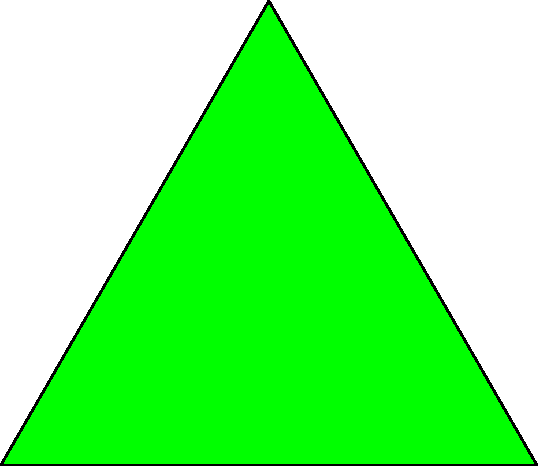
\includegraphics[width=0.2\textwidth]{figures/triangle.pdf}}\hspace{2cm}
	\subfigure[Un carré.]{\label{fig:Carre}
\includegraphics[width=0.2\textwidth]{figures/carre.pdf}}
	\caption{\label{fig:TriCar}Un carré et un triangle.}
\end{figure}
À la figure \ref{fig:TriCar}, le triangle \subref{fig:Triangle} et le carré \subref{fig:Carre} ont été placés côtes-\`a-côtes grâce \`a la commande \verb|\subfigure|. 



%%%%%%%%%%%%%%%%%%%%%%%%%%%%%%%%%%%%%
%%   BIBLIOGRAPHIE                  %
%%%%%%%%%%%%%%%%%%%%%%%%%%%%%%%%%%%%%
  % Enlever les commentaires de la prochaine commande si vous préférez que le
  % chapitre s'appelle « Références » plutôt que « Bibliographie » (au choix selon le contexte).
%\let\bibname=\refname   

%% Lorsque vous serez prêt à faire afficher votre bibliographie
%% et vos références, enlevez les commandaires des commandes suivantes
%% et donnez le nom de votre fichier .bib à la commande \bibliography{..}
%% (consultez l'exemple au besoin).  Vous pouvez utiliser le style de votre
%% choix.  Le fichier francaissc.bst est inclus avec le gabarit.  Vous pouvez
%% utiliser ce style avec  \bibliographystyle{francaissc}
% 
\bibliographystyle{francaissc}		    % Le style de la bibliographie. Notons que les extensions ne sont pas données pour ces deux fichiers.
\bibliography{references}		    % La base de données contenant des entrées bibliographiques. Seules celles référencées dans le texte seront ajoutées \`a la bibliographie.


%
% ----------  A N N E X E S  ----------
%

%%% Enlever le commentaire de \appendix pour faire vos annexes.
%%% Les annexes sont ensuites faites comme un chapitre normal : \chapter{nom_de_l'annexe}.
\appendix
\chapter{Le titre}

\section{Section un de l'annexe A}

La premi\`ere annexe du document.

Pour plus de renseignements, consultez le site \href{http://www.fesp.umontreal.ca}{web de la FESP}.
\begin{table}[htb]
	\renewcommand{\arraystretch}{1.25}
	\newcommand{\dotrule}[1]{\parbox[t]{#1}{\dotfill}}
	\centering
	\caption[Titre alternatif pour la table des mati\`eres]{Liste des parties}
	\label{tab:parties}
	\begin{tabular}{p{0.6\textwidth}@{\hspace{0.15\textwidth}}p{0.15\textwidth}}
		\hline\hline & \\[-3mm]
  		Les couvertures conformes 											& obligatoires			\\
		Les pages de garde 													& obligatoires			\\
		La page de titre 													& obligatoire			\\
		Le résumé en français et les mots clés français						& obligatoires			\\
		Le résumé en anglais et les mots clés anglais 						& obligatoires			\\
		Le résumé de vulgarisation											& facultatif			\\
		La table des mati\`eres, la liste des tableaux, la liste des figures 	& obligatoires			\\
		La liste des sigles, la liste des abréviations						& obligatoires			\\
		La dédicace															& facultative			\\
		Les remerciements 													& facultatifs			\\
		L'avant-propos 														& facultatif			\\
		Le corps de l'ouvrage												& obligatoire			\\
		L'index analytique													& facultatif			\\
		Les sources documentaires 											& obligatoires			\\
		Les appendices (annexes) 											& facultatifs			\\
		Le curriculum vit\ae{}												& facultatif			\\
		Les documents spéciaux 												& facultatifs			\\
		[3mm] \hline\hline
	\end{tabular}
\end{table}
Pour plus de renseignements, consultez le site \href{http://www.fesp.umontreal.ca}{web de la FESP}.

\chapter{Le titre2}
\chapter{Le titre3}
\chapter{Le titre4}

\end{document}
